\chapter{Clustering}

In the field of clustering analysis, there is no strict definition for a cluster itself. That may be one reason why there is such a vast amount of clustering algorithms; many authors such as \citet{estivill2002so} discuss this topic.  However, the~one think in common that we can find among all the algorithms is a work with a~group of data objects.


According to a field of use, the data objects are represented variously (graphs, text sequences, etc.). The current thesis will focus on a clustering of objects represented by a vector of real numbers.

Suppose a dataset $\mathcal{D}$ given as a $n$ $d$-dimensional vectors $(x_1,\dots,x_d) \subset \R^d$  --- objects; each element of a vector describes a specific object property. Two objects are similar if values of their respective properties are alike. Then, a clustering analysis can be defined as a form of an object grouping into subsets of $\mathcal{D}$ that maximizes the inter-set object similarity and minimizes the intra-set object similarity.

\section{Clustering models}

Specific variations of clustering analysis are defined by a clustering model. For the purpose of the following chapters, we will describe these two clustering models:
\begin{itemize}
	\item Centroid-based model
	\item Hierarchical model
\end{itemize}


\subsection{Centroid-based model}

\emph{The centroid-based clustering model} represents clusters only by a central vector --- \emph{centroid} --- which is not necessarily a member of a dataset.

\begin{defn}[Centroid]
	Suppose a cluster $\mathcal{C} \subset \R^d$. We define the \emph{centroid} $c \in \R^d$ of the cluster $\mathcal{C}$ such that its $i$-th element is equal to the arithmetic mean of the $i$-th elements of all points $o \in \mathcal{C}$. 
	\label{def01:centr}
\end{defn}

Many~implementations of this model need the number of required centroids in advance (denoted by $k$). We define the following optimalization problem for~this kinds of~algorithms: 

\begin{problem}[Centroid-based clustering]
	Having a distance function $d$, find $k$ centroids $C_1,\dots,C_k$ from the domain of the dataset $\mathcal{D}$ such that the sum \ref{eq01:sum}
	is minimized.
\end{problem}

\begin{equation}\label{eq01:sum}
	\sum_o^{\mathcal{D}} \min_{i=1\dots k}d(o,C_i)
\end{equation}

This problem is uneasy to solve due to its exponential complexity. Hence, many approximation algorithms emerged. 

\subsubsection{k-means}

The most common implementation of a centroid-based clustering is \emph{k-means}. Its algorithm can be expressed in a few simple steps (see alg.~\ref{alg01:kmeans}).

\begin{algorithm}
	\caption{$k$-means clustering}
	\label{alg01:kmeans}
	\begin{algorithmic}[1]
		\Procedure{$k$-means}{$k\in\R$, $\mathcal{D} \subset \R^d$, $d \in \R^d \times \R^d \to \R$}
		\State $\mathcal{C} \gets$ first $k$ objects from  $\mathcal{D}$ \Comment{select initial centroids}
		\Repeat
			\For{$i \in \{1\dots k\}$}
				\State $K_i \gets \{\}$\Comment{create empty clusters}
			\EndFor
			\ForAll{$o \in \mathcal{D}$}
				\State $j \gets$ index of the closest centroid $c_j \in \mathcal{C}$ to $o$; $d(o,c_j)$ is minimal
				\State $K_{j} \gets K_{j} \cup o$ \Comment{assign objects to clusters}
			\EndFor
			\For{$i \in \{1\dots k\}$}
				\State $c'_i \gets$ centroid of $K_i$ \Comment{compute new centroids}
			\EndFor
			\State $\mathcal{C}' \gets \{c'_1,\dots,c'_k\}$
			\State swap $\mathcal{C}$ and $\mathcal{C}'$
		\Until{$\mathcal{C} = \mathcal{C}^\prime$}
		\State \textbf{return} $\mathcal{C}$
		\EndProcedure
	\end{algorithmic}
\end{algorithm}


The algorithm divides data into $k$ clusters (hence, \emph{k}-means) in a iterative manner. Before the first iteration, initial $k$ central vectors are selected from the~dataset (we chose the first $k$ objects; however, the way of selecting $k$ initial vectors varies between 
implementations). In the iteration loop, dataset objects are grouped into clusters according to the closest centroid. After that, new centroids are then computed from new clusters. Next iteration follows until centroids does not change or predefined number of iterations is reached. 

The $k$-means algorithm is easily comprehensible; hence can be employed in a large variety of datasets. Moreover, the algorithm simplicity favors in its great performance. However, the disadvantages are inability to deal with the noise in a dataset and clusters of non-convex shape~\cite{uppada2014centroid}.
  

\subsection{Hierarchical model}

In the \emph{hierarchical clustering model}, objects are \emph{connected} together forming tree-like structure. In contrast with the aim of a centroid-based model that returns only $k$ centroids, hierarchical clustering algorithms capture whole connecting process. These algorithms starts with all objects from a dataset as initial clusters. Each iteration, two clusters are connected creating a new one, finishing with one all-inclusive cluster. Commonly, the algorithms represent the connecting process as an ordered list of pairs --- a list of connected clusters~\cite{karypis1999chameleon}.

The above described approach of a hierarchical algorith is called \emph{agglomerative} approach. An agglomerative algorithm begins with each object representing a cluster on its own. Then, in a bottom-up fashion, clusters are successively connected into the only cluster. The other option is \emph{divisive approach}. Beginning with a single all-inclusive cluster it is divided into sub-clusters until single objects remain~\cite{rokach2005clustering}. 

The result of a hierarchical clustering can be viewed in a \emph{dendrogram} (see fig.~\ref{fig01:dendro}). The x-axis states the distance between connected clusters. The y-axix shows labels of the objects from a dataset. Hence, the clusters that are connected in the higher part of the dendrogram were further apart from each other, and the~clusters connected at its bottom were close to each other.

\begin{figure}\centering
	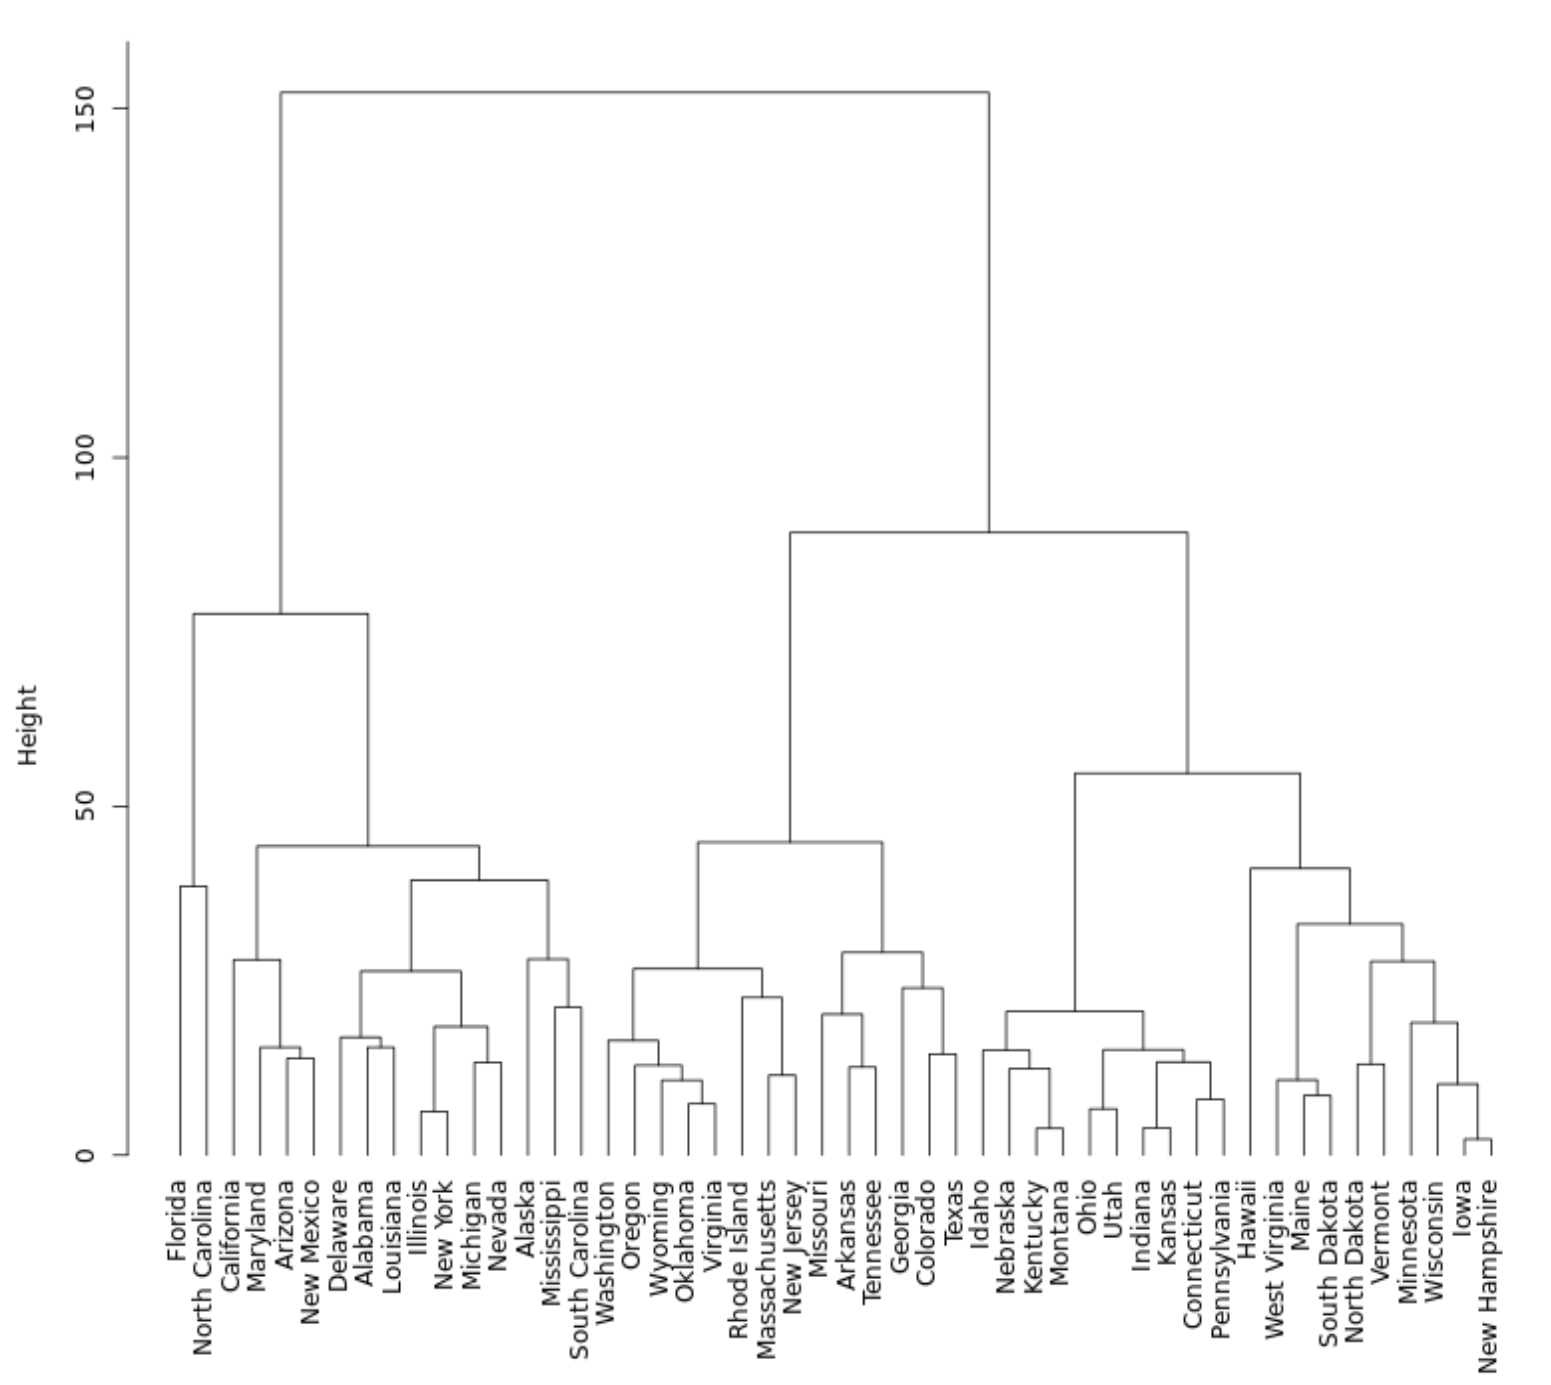
\includegraphics[width=10.5cm]{img/dendro}
	\caption{An example of a dendrogram.}
	\label{fig01:dendro}
\end{figure}

To know which two clusters are connected (or respectively, how a cluster is~divided into two), algorithms use a \emph{measure of a dissimilarity} between clusters.  
A~hierarchical clustering model distinguishes various kind of algorithms based on~the~choice of this measure. Commonly, the computation of the measure is~dependent on the two factors: a \emph{distance function} and a \emph{linkage criterion}. 

\subsubsection{Distance functions}

A \emph{distance function} is used on objects of a dataset to express how far they are~from each other in the observed domain. Supposing objects are represented as vectors $v \in \R^d$, variations of \emph{Minkowski distance formula} (see eq.~\ref{eq01:mink}) are the most commonly used.
They are \emph{Manhattan distance} ($p=1$), \emph{Euclidean distance} ($p=2$) and \emph{Chebyshev distance} ($p \to \infty$) (see tab.~\ref{tab01:mink}).

It is obvious that the choice of a distance function can influence the result of a clustering. Hence, it should be chosen with respect to the properties of a provided dataset. \citet{aggarwal2001surprising} show the qualitative behavior of different distance functions in the $k$-means algorithm.  

\begin{equation}\label{eq01:mink}
||a-b||_p = (\sum_{i=1...d}|a_i-b_i|^p)^{\frac{1}{p}}
\end{equation}

\begin{table}
	\centering
	\begin{tabular}{ll}
		\toprule
		Distance measure & Formula \\
		\midrule
		Manhattan & $||a-b||_1 = \sum_{i=1...d}|a_i-b_i|$          \\
		Euclidean & $||a-b||_2 = \sqrt{\sum_{i=1...d}(a_i-b_i)^2}$ \\
		Chebyshev & $||a-b||_\infty = \max_{i=1\dots d}|a_i-b_i|$  \\ \bottomrule
	\end{tabular}
	\caption{Variations of Minkowski distance formula.}
	\label{tab01:mink}
\end{table}

\subsubsection{Linkage criteria}

As the reader may have already discovered, one particular problem arises. A~hierarchical algorithm can not compute a proximity of two clusters only by using distance function as it is the function of \emph{dataset objects}. Hence, we define a~function of \emph{object clusters} to complete the process of measuring dissimilarity; a~\emph{linkage criterion}. Given clusters $A$ and $B$ as sets of dataset objects and a distance function~$d$, we define the following \emph{linkage criteria}~\cite{yim2015hierarchical}:

\begin{description}
	\item[Single linkage] -- Also referred to as a minimum method, a \emph{single linkage criterion} computes the distance between $A$ and $B$ as the minimum distance between all pairs $(a,b) \in A\times B$ (see eq.~\ref{eq01:single_link}).
	\begin{equation}\label{eq01:single_link}
	\min\{d(a,b) : a \in A, b \in B\}
	\end{equation}
	
	The major drawback this criterion suffers is a \emph{cluster chaining}. Such two clusters can be connected that they do not share any other pair of close proximity objects than the one that determined the connection. This produces long thin clusters with a great distance between some objects.
	
	\item[Complete linkage] -- Also referred to as a maximum method, a \emph{complete linkage criterion} is similar to the single linkage criterion. But as opposed to~finding the minimum, this criterion uses the maximum of object pairs for the~computation of a cluster dissimilarity (see eq.~\ref{eq01:complete_link}). 
	\begin{equation}\label{eq01:complete_link}
	\max\{d(a,b) : a \in A, b \in B\}
	\end{equation}
	
	The criterion suffers from its simplicity as well as the single linkage. But~instead of naively connecting dissmimilar clusters, here simmilar clusters are~not connected in some cases. Having all objects pairs in a close proximity to each other but one object being rather far from the others, the~criterion will not link the clusters as the maximum distance deteriorates the rest.
	
	\item[Centroid linkage] -- A \emph{centroid linkage criterion} tries to solve the problems of the~aforementioned criteria by measuring the distance between the centroids of clusters. It~introduces a form of an average into the computation; the think that the criteria above lack.
\end{description}

A choice of a linkage criterion in hierarchical clustering algorithm is vital. As~stated above, it can change the course of clustering in a great manner. Chosen improperly, it can have a disastrous effect on the final result.

\begin{figure}\centering
	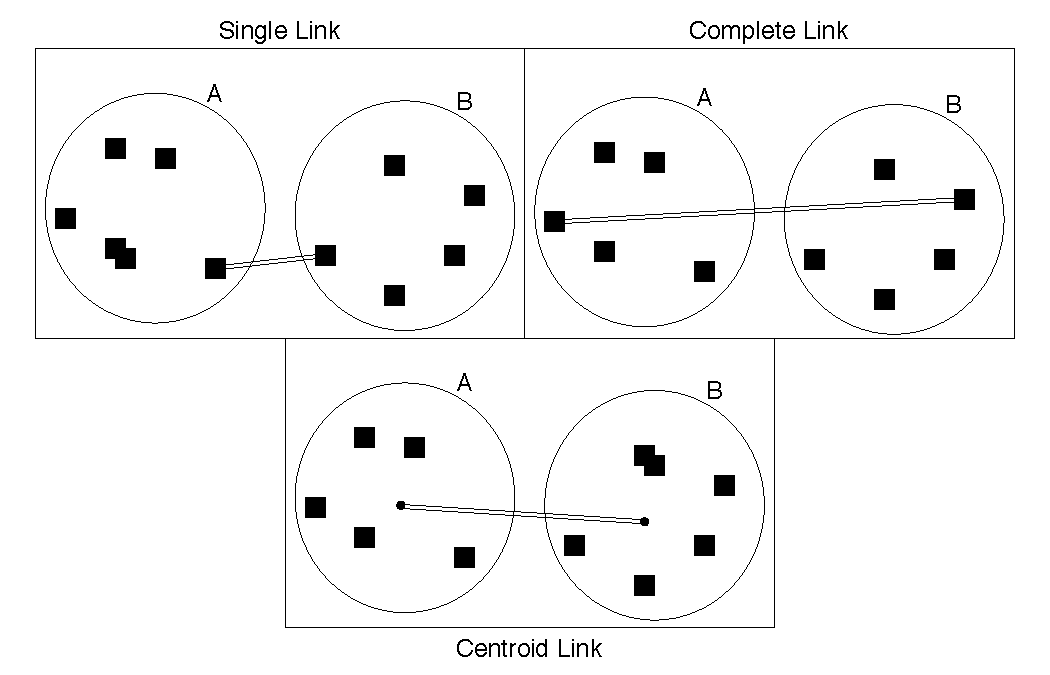
\includegraphics[width=10cm]{img/linkage_criteria}
	\caption{An example of three linkage criteria. The double line represents the distance between clusters A and B according to the respective criterion.}
	\label{fig01:link}
\end{figure}

\section{Mahalanobis-based clustering}

To produce more meaningful results, hierarchical clustering algorithms have branched into many variations; each focusing on a specific dataset type. The~\emph{Ma\-ha\-la\-no\-bis-based hierarchical clustering analysis} (MHCA) focuses on datasets that create clusters of ellipsoid shapes. This datasets are common products during natural measurements of cell cytometry data in bio-informatics.

\subsection{Mahalanobis distance}

The significant part of this clustering variation is the measure of cluster dissimilarity. It is based on the \emph{Mahalanobis distance}~\cite{mahalanobis1936generalized}, a distance between a point and a set of points (in our case a cluster). If points in the set are strongly correlated in some axis, then points laying on this axis are closer to the set than points that are not; even if their euclidean distance to the center of the set is closer.

For its computation, the Mahalanobis distance uses a covariance matrix of the~participating cluster. To know how the matrix is created, we need to define the \emph{random vector of a cluster}. 

\begin{defn}[Random vector]
	Given a cluster of $d$-dimensional points $\mathcal{C} \subset \R^d$, we define the \emph{random vector} $v$ of the cluster $\mathcal{C}$ as a vector of $d$ discrete random variables; a random variable $v_i$ has equal probability values $\{o_i:o\in \mathcal{C}\}$
\end{defn}

With the random vector of a cluster we can easily create the covariance matrix of a cluster and properly define the Mahalanobis distance:

\begin{defn}[Mahalanobis distance]
	Having a cluster of $d$-dimensional points $\mathcal{C} \subset \R^d$, its centroid $c$ and the covariance matrix $\mathcal{S}$, we define the \emph{Mahalanobis distance} between $u \in \R^d$ and $\mathcal{C}$ by the equation \ref{eq01:maha}.
	\begin{equation}\label{eq01:maha}
	d_M(u,\mathcal{C}) = \sqrt{(u-c)^TS^{-1}(u-c)}
	\end{equation}
	\label{def01:maha}
\end{defn}


However, using the equation \ref{eq01:maha}, we are only able to compute a point-cluster proximity. To fully incorporate the distance in a hierarchical algorithm, we need to find a method how to measure cluster-cluster proximity. There are two options how to achieve this:

\begin{itemize}

\item
First, we can choose a path of the single and complete linkage criterion; hence, all points in cluster contribute to the measure. We achieve this with~the~\emph{Full Mahalanobis distance} (FMD):

\begin{defn}[Full Mahalanobis distance]
	Having clusters $\mathcal{C}$ and $\mathcal{C}'$, we define the \emph{Full Mahalanobis distance} between clusters $\mathcal{C}$ and $\mathcal{C}'$ as the arithmetic mean of the Mahalanobis distances between each object $o \in \mathcal{C}$ and the~cluster $\mathcal{C}'$ (see eq.~\ref{eq01:fmd}).
	\begin{equation}\label{eq01:fmd}
	d_{FM}(\mathcal{C},\mathcal{C}') =\frac{1}{|\mathcal{C}|}\sum_{o\in\mathcal{C}}{d_M(o,\mathcal{C}')}
	\end{equation}
	\label{def01:fmd}
\end{defn}

\item
The second option is similar to the centroid linkage as only the centroid of a cluster takes part in the computation. We define this as the \emph{Centroid Mahalanobis distance} (CMD):

\begin{defn}[Centroid Mahalanobis distance]
	Suppose we have a cluster $\mathcal{C}$ with its centroid $c$ and a cluster $\mathcal{C}'$. We define the \emph{Centroid Mahalanobis distance} between clusters $\mathcal{C}$ and $\mathcal{C}'$ as the Mahalanobis distance between $c$ and $\mathcal{C}'$ (see eq.~\ref{eq01:cmd}).
	\begin{equation}\label{eq01:cmd}
	d_{CM}(\mathcal{C},\mathcal{C}')=d_M(c,\mathcal{C}')
	\end{equation}
	\label{def01:cmd}
\end{defn}

\end{itemize}

To illustrate the measure of the Mahalanobis distance, let us suppose we have two elliptic clusters. In the means of the proximity, the measure favors such clusters that their ellipsis are alongside rather than in a prolongation of one another~\cite{dagnelie1991using} (see fig.~\ref{fig01:ellipses}). Only when the objects of a cluster form a spherical shape, this measure of dissimilarity is proportional to the euclidean distance with a corresponding linkage.

\begin{figure}\centering
	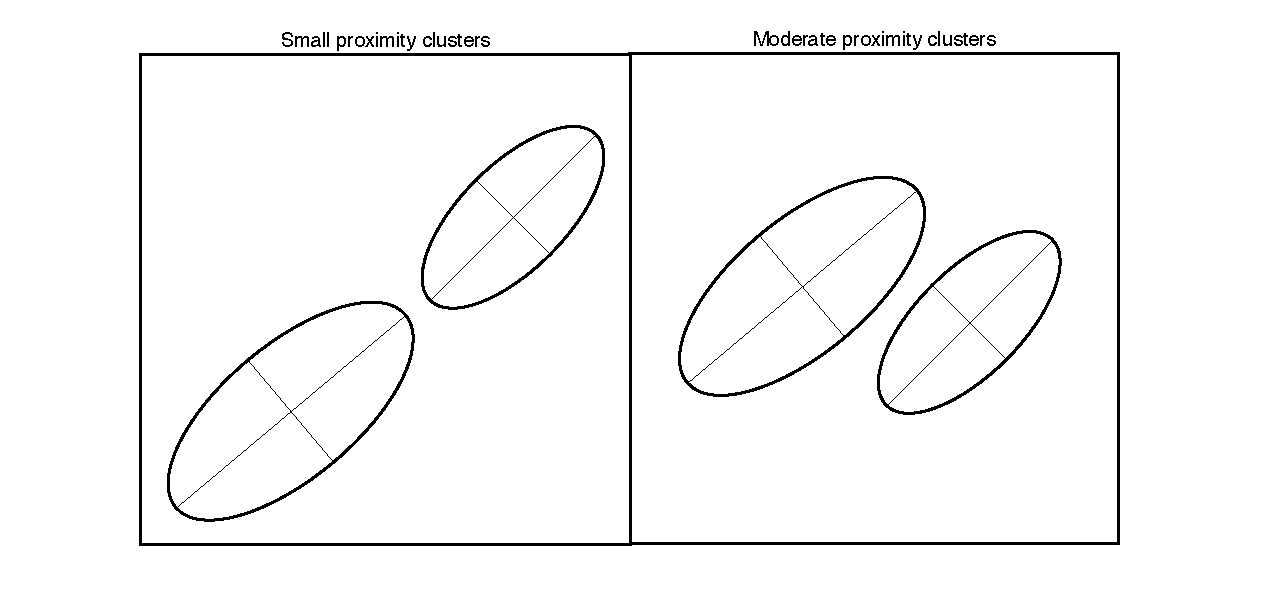
\includegraphics[width=10cm]{img/ellipses}
	\caption{An example of the cluster dissimilarity in the Mahalanobis-based hierarchical clustering.}
	\label{fig01:ellipses}
\end{figure}



The pros and cons between FMD and CMD are trivial. Due to the full point contribution, FMC can produce more precise measure than its counterpart. On the~other hand, CMD compensates it with much lower time complexity.

\vspace{0.5cm}

To make use of these Mahalanobis distance variants in MHCA implementations, we need the distance function to be \emph{symmetric}. Originally, the Mahalanobis distance is not a symmetric funtion. However, we easily achieve this attribute with the \emph{Generalized distance}.

\begin{defn}[Generalized distance]
	Given clusters $\mathcal{C}$, $\mathcal{C}'$ and a variant of~the~Mahalanobis distance~$d$ (either FMD or CMD), we define the \emph{Generalized distance} between clusters $\mathcal{C}$ and $\mathcal{C}'$ as the arithmetic mean of distances between $\mathcal{C}$, $\mathcal{C}'$ and $\mathcal{C}'$, $\mathcal{C}$ (see eq.~\ref{eq01:gene}).
	\begin{equation}\label{eq01:gene}
	d_G(\mathcal{C},\mathcal{C}') = \frac{d(\mathcal{C},\mathcal{C}')+d(\mathcal{C}',\mathcal{C})}{2}
	\end{equation}
	\label{def01:gene}
\end{defn}  


\subsection{Algorithm behavior improvemets}

If the distance function of a MHCA implementation was let to be a pure Mahalanobis distance, it would eventually halt due to the following problem --- the covariance matrix computation.

In early stages of MHCA --- when clusters consist of fewer points --- the covariance matrix of a cluster is often singular. Hence, we can not compute its inverse and perform the distance measure. Furthermore, the matrix can happen to be close to singular and --- when inverted --- can produce distorted results.

To solve this problem, we used the variant of the~euclidean distance with the~centroid linkage on clusters whose size are under a~specified threshold --- the~\emph{Mahalanobis threshold}. The value of the threshold is proportional to the size of a dataset varying at about 0.1\% of the dataset size~\cite{fivser2012detection}. Hence, to implement this optimization we defined the \emph{Altered general distance}.

\begin{defn}[Altered general distance]
	Given a threshold $T_M$, a cluster $\mathcal{C}$ with~its centroid $c$, a cluster $\mathcal{C}'$ with~its centroid $c'$ and a variant of the Mahalanobis distance $d$, we define the \emph{Altered general distance} by equation \ref{eq01:alt}:
	\begin{equation}
	d_A(\mathcal{C},\mathcal{C}')=
	\begin{cases}
	d_G(\mathcal{C}, \mathcal{C}'), & \text{if $|\mathcal{C}|\ge T_M$ and $|\mathcal{C}'|\ge T_M$},\\
	\dfrac{d(\mathcal{C}, \mathcal{C}')+||c-c'||_2}{2}, & \text{if $|\mathcal{C}| < T_M$ and $|\mathcal{C}'|\ge T_M$},\\
	\dfrac{||c-c'||_2+d(\mathcal{C}', \mathcal{C})}{2}, & \text{if $|\mathcal{C}|\ge T_M$ and $|\mathcal{C}'|< T_M$},\\
	||c-c'||_2, & \text{if $|\mathcal{C}|< T_M$ and $|\mathcal{C}'|< T_M$}.\\
	\end{cases}
	\label{eq01:alt}
	\end{equation}
	\label{def01:alt}
\end{defn}



\section{Algorithm complexity}

The common problem in clustering algorithms is their time complexity. In hierarchical clustering algorithms, we can achieve time complexity of $O(n^3)$ using $O(n^2)$ space. However, this restricts the use of the algorithms; datasets must consist of $10^3$ to $10^5$ points when using a contemporary hardware. Note that this restrictions is present not only due to the time complexity; for the current computers, it would be a difficult task to store $10^6$ data points into a structure with quadratic space requirements (i.e. a matrix).

Due to the consequences of this problem, a MHCA algorithm implementation must be created wisely. \citet{day1984efficient} help us with this task by~proposing three different implementations of a hierarchical clustering analysis (HCA). We describe them thoroughly and research potential pros and cons they bring:

\begin{description}
	\item[HCA with the dissmilarity matrix] -- The first and the most trivial implementation uses the \emph{dissimilarity matrix} $M$.
	
	\begin{defn}[Dissimilarity matrix]
		Suppose a dataset $\mathcal{D}$ divided into clusters $C_1,\dots,C_m$ and a function $d$ as a measure of dissimilarity. Then, the~\emph{dissimilarity matrix} $M$ is $m\times m$ matrix where $M_{ij} = d(C_i,C_j)$.
		\label{def01:dismat}
	\end{defn}

 Unless there remains only one cluster, the algorithm searches $M$ for the closest pair of clusters, stores the pair and updates $M$ (see alg.~\ref{alg01:dismat}).
	
	\begin{algorithm}
		\caption{HCA with dissimilarity matrix}
		\label{alg01:dismat}
		\begin{algorithmic}[1]
			\Procedure{dismat}{$\mathcal{D} \subset \R^d$}
			\State initialize the dissimilarity matrix $M$
			\For{$k=|\mathcal{D}|$ \textbf{downto} $1$}
			\State search $M$ for the closest pair $(i,j)$ \Comment{time: $O(k^2)$}
			\State store cluster pair $(i,j)$ into the merge list \Comment{time: $O(1)$}
			\State update $M$ \Comment{time: $O(k)$}
			\EndFor
			\State \textbf{return} list of merged clusters
			\EndProcedure
		\end{algorithmic}
	\end{algorithm}

	The main cycle in line $3$ repeats $n = |\mathbb{D}|$ times; each iteration the number of clusters is reduced by 1. The search in line $4$ is bounded by $O(n^2)$ time, having its peak in the first iteration when $k=n$. The update in~line~$6$ reflects the deletion of clusters $i$ and $j$ and the addition of the new one. Hence, it needs to perform $k$ new dissimilarity measures for the new cluster (bounded by $O(n)$ during the first iteration as well). As there are $n$~iterations performed, this results in the overall time complexity of $O(n^3)$. 
	
	The space required to store $M$ is $O(n^2)$. As there is no other non-trivial requirement, the overall space complexity is $O(n^2)$. 
	\begin{rem}
		However, there is no need to store the matrix at all. We can choose to measure a cluster dissimilarity \emph{in-place}. Line $6$ would become redundant and the time complexity of line $4$ would increase by a constant multiplicative factor; hence, the overall time complexity remains the same while the~space complexity becomes $O(n)$.
	\end{rem}
	

	\item[HCA with the nearest neighbor array] -- This algorithm introduces the array of the nearest neighbor.
	
	\begin{defn}[Nearest neighbor array]
		Suppose a dataset $\mathcal{D}$ divided into clusters $C_1,\dots,C_m$ and a function $d$ as a measure of dissimilarity. Then, the~\emph{nearest neighbor array} $N$ is a $m$-element array of indices $\{1,\dots,m\}$ where each element $N_i$ satisfies the equation \ref{eq01:neigh}:
		\begin{equation}
		d(C_i,C_{N_i}) = \min\{d(C_i,C_j) : j \in \{1,\dots,m\} \setminus \{i\}\}
		\label{eq01:neigh}
		\end{equation}
		
		\label{def01:neigh}
	\end{defn}
	
	 Instead of the dissimilarity matrix, each cluster is assigned the index of the~closest neighboring cluster (see alg.~\ref{alg01:neigh}). 
	 Compared to the alg.~\ref{alg01:dismat}, this algorithm trades the expensive \emph{closest pair search} with the expensive \emph{structure update}.
	
	
	
	\begin{algorithm}
		\caption{HCA with the nearest neighbor array}
		\label{alg01:neigh}
		\begin{algorithmic}[1]
			\Procedure{neighbor}{$\mathcal{D} \subset \R^d$}
			\State initialize $N$
			\For{$k=|\mathcal{D}|$ \textbf{downto} $1$}
			\State search $N$ for the closest pair $(i,j)$ \Comment{time: $O(k)$}
			\State store cluster pair $(i,j)$ into the merge list \Comment{time: $O(1)$}
			\State update $N$ \Comment{time: $O(k^2)$}
			\EndFor
			\State \textbf{return} list of merged clusters
			\EndProcedure
		\end{algorithmic}
	\end{algorithm}
	
	
	 In line $4$, each closest pair search can be performed in $O(n)$ time as the~array length does not exceeds $n$ elements. However in line $6$, the worst case update of $N$ happens when every cluster is in the closest neighborhood with the clusters that are being merged; the clusters of indices $i$ and $j$. In this case, the whole array has to be recomputed, which corresponds to~the~computation of the whole dissimilarity matrix. Hence, the time complexity for this step is $O(n^2)$. The overall time complexity is $O(n^3)$. The space complexity is $O(n)$ as $N$ does not have more than linear space requirements.
	 
	 \begin{rem}
	 	Despite equal time complexities, this algorithm may outperform the previous one as in the majority of situations the update step in line $6$ does not require the whole array to be recomputed. Moreover, if the~number of elements to be updated remains constant each iteration, the overall algorithm time complexity may be $O(n^2)$. 
	 \end{rem}
	 
	 \item[HCA with priority queues] -- This algorithm takes the advantage of the previous one employing the fast search and combines it with the fast update using \emph{priority queues} (see alg.~\ref{alg01:queue}).
	 Each object from a dataset is assigned a~priority queue constructed from the remainder of the datset. The priority label of a queued element is a dissimilarity measure between the object and the queued element. 
	 
	 \begin{algorithm}
	 	\caption{HCA with priority queues}
	 	\label{alg01:queue}
	 	\begin{algorithmic}[1]
	 		\Procedure{queues}{$\mathcal{D} \subset \R^d$}
	 		\ForAll{$o \in \mathcal{D}$}
	 		\State initialize a priority queue from $\mathcal{D} \setminus \{o\}$
	 		\EndFor
	 		\For{$k=|\mathcal{D}|$ \textbf{downto} $1$}
	 		\State search $k$ queues for the closest pair $(i,j)$ \Comment{time: $O(k)$}
	 		\State store cluster pair $(i,j)$ into the merge list \Comment{time: $O(1)$}
	 		\State update $k$ priority queues \Comment{time: $O(k\log{k})$}
	 		\EndFor
	 		\State \textbf{return} list of merged clusters
	 		\EndProcedure
	 	\end{algorithmic}
	 \end{algorithm}
 
 	
 	As an operation of retrieving a minimum in a priority queue has $O(1)$ time complexity, the search step in line $4$ takes $O(k)$ time (bounded by $O(n)$ during the first iteration). Next in line $6$, we need two delete and one insert operations (corresponding to deleting two merged clusters and inserting one new). As these operations require $O(\log{n})$ time, we can update $n$ queues in $O(n\log{n})$ time.
 	
 	To sum up, the overall time complexity is $O(n^2\log{n})$. The space complexity is back to $O(n^2)$ due to the linear space requirements of a queue.
 	
 	\begin{rem}
 		Note that this is the only algorithm from the three described that unavoidably requires quadratic space. This may lead to the further restrictions of its usage for large datasets.
 	\end{rem}

\end{description}

To fully show disadvantages of the algorithm complexity, we measured a R language library function \texttt{hclust}; a frequenly used implementation of HCA. It computes the centroid linkage with the euclidean distance and uses the dissimilarity matrix. 

Fig. \ref{fig01:hclust} shows above mentioned polynomial time complexity of the implementation. Moreover, it halted at a dataset size of 47K as the testing machine \footnote{Intel Core i9-8950HK, 32GB RAM} ran out of memory.

In conclusion, the space complexity of HCA can be even more restrictive in the means of the overall algorithm usability than its time complexity. We solve this by removing high space complexity structures (such as the dissimilarity matrix) for the price of a lower speed while retaining the same asymptotic time complexity.

\begin{figure}\centering
	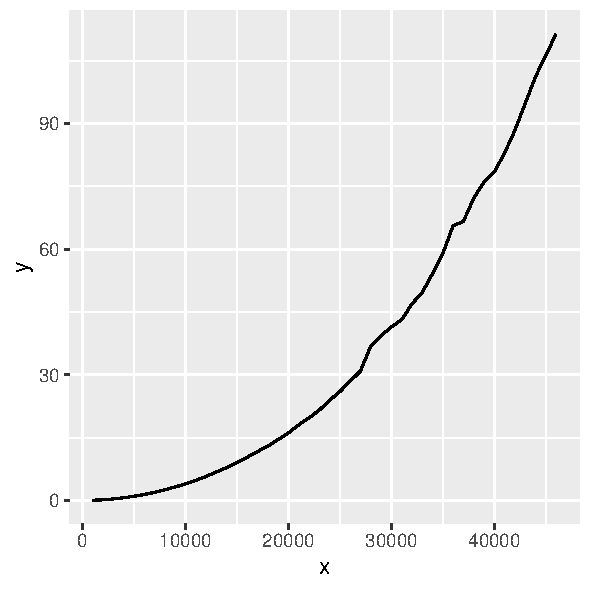
\includegraphics[width=10cm]{img/hclust}
	\caption{A time complexity of \texttt{hclust} with respect to the size of a dataset.}
	\label{fig01:hclust}
\end{figure}
